\chapter{Caso de estudio}

En este capítulo se va a realizar un ejemplo de uso de la interfaz para la detección de anomalías en red con unos datos previamente anonimizados de una red corporativa real.

\bigskip

Primero se comenzará a hacer un análisis de todos los ficheros de datos como un único modelo y posteriormente en modelos separados de cada uno de los mismos. La figura 10.1 muestra la configuración utilizada para el primer análisis.

\bigskip

\begin{figure}[H]
\centering
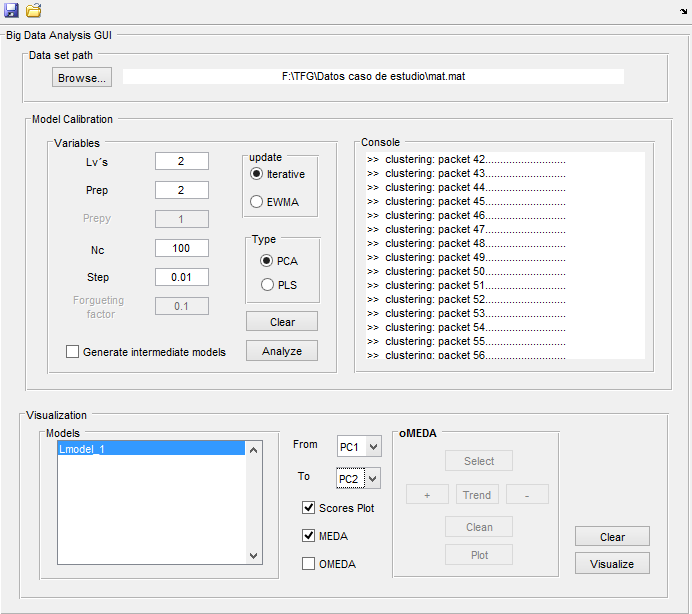
\includegraphics[width=0.7\textwidth]{imagenes/casoEstudio/10_1.png}
\caption{GUI para un solo modelo.}
\end{figure}

\begin{figure}[!ht]
\centering
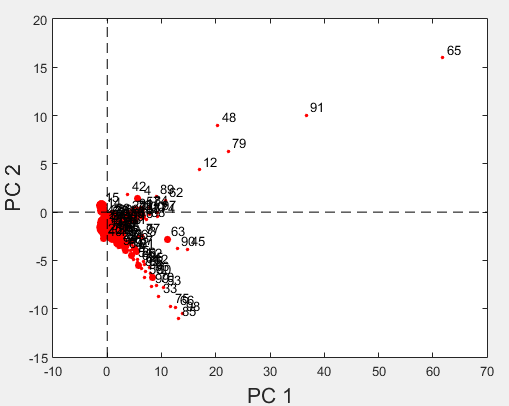
\includegraphics[width=0.7\textwidth]{imagenes/casoEstudio/10_2.png}
\caption{Score plot un modelo.}
\end{figure}

\bigskip

En la figura 10.2 se puede apreciar cómo hay varias observaciones que se salen de la concentración normal de datos, estos \textbf{outliers} pueden darnos información sobre una posible anomalía en el funcionamiento normal de la red.

\begin{figure}[H]
\centering
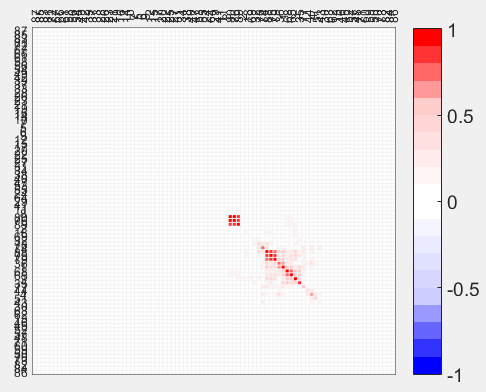
\includegraphics[width=0.7\textwidth]{imagenes/casoEstudio/10_3.png}
\caption{MEDA un modelo.}
\end{figure}

\bigskip

Las observaciones 65, 91, 48, 79 y 12 parecen no estar dentro de los "limites" que siguen el resto de las mismas, por lo que se van a estudiar más en profundidad. Para esto en el gráfico MEDA de la figura 10.3 se observa en términos generales el funcionamiento de la red, viendo las relaciones existentes entre variables. Posteriormente con oMEDA se verán las relaciones entre variables y observaciones.

\begin{figure}[!ht]
\centering
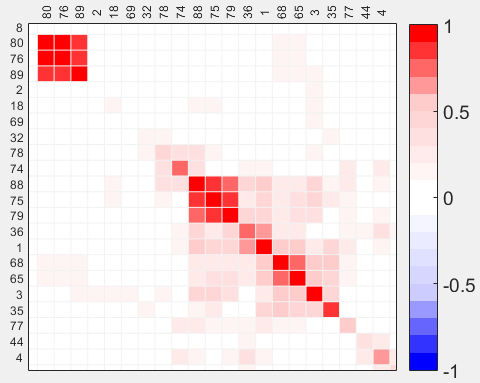
\includegraphics[width=0.7\textwidth]{imagenes/casoEstudio/10_4.png}
\caption{MEDA un modelo con zoom.}
\end{figure}

\bigskip

En la figura 10.4 se puede ver el gráfico MEDA ampliado en la zona donde existen relaciones para poder ver qué variables son las relacionadas. En Dicha figura se pueden observar las relaciones existentes entre variables quedando fuertemente relacionadas 4 grupos de variables. El primer grupo son las variables 80, 76 y 89. El segundo grupo son las variables 88, 75 y 79. El tercero las variables 36 y 1. Y el último 68 y 65. El contenido de las variables se muestra en la tabla 10.1. El primero de los 3 grupos mostrados en la tabla nos indica que en conexiones con paquetes de datos de gran tamaño el estado de la conexión se mantiene abierto durante todo el periodo de tiempo que ha durado la captura. El segundo muestra que en términos generales cuando los paquetes son de tamaño medio la conexión se cierra dentro del periodo de captura. El tercero nos dice que cuando el puerto de origen es privado la IP también lo es.

\begin{table}[H]
\begin{center}
\begin{tabular}{|c|c|c|}
\hline
\textbf{Variable} &\textbf{Nombre} & \textbf{Descripción} \\
 \hline \hline

89 & nf\_state\_open & Estado de conexión abierta	\\ \hline
80 & nf\_dbyte\_long & Paquetes de destino de gran tamaño \\ \hline
76 & nf\_sbyte\_long & Paquetes de origen de gran tamaño  \\	
\hline \hline

88 & nf\_state\_close & Estado de conexión cerrada	\\ \hline
79 & nf\_dbyte\_medium & Paquetes de destino de tamaño medio	\\ \hline
75 & nf\_sbyte\_medium & Paquetes de origen de tamaño medio\\
 \hline \hline

36 & nf\_sport\_private & Puerto de origen privado\\ \hline
1 & nf\_sip\_private & IP privada de origen	\\
\hline \hline

68 & nf\_dport\_register & Puerto de destino mayor a 1024\\ \hline 
65 & nf\_dport\_8089 & Puerto de destino 8089 \\ \hline 
\end{tabular}
\caption{Contenido variables.}
\end{center}
\end{table}

\bigskip

Ahora que ya se conoce el contenido de las variables mas relacionadas se pasa a crear un gráfico oMEDA con los outliers para poder relacionar variables con observaciones y poder encontrar dónde se producen las anomalías. En la figura 10.5 se ve como se marcan las observaciones outliers.

\begin{figure}
\centering
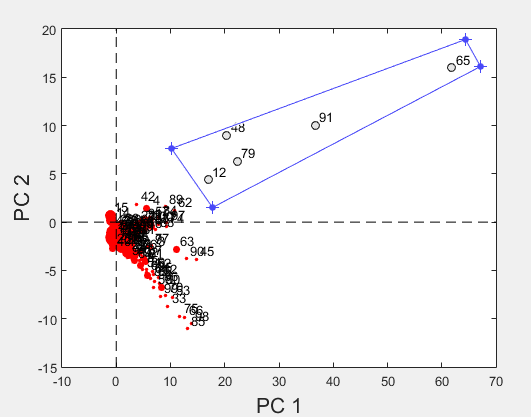
\includegraphics[width=0.7\textwidth]{imagenes/casoEstudio/10_5.png}
\caption{Observaciones marcadas para oMEDA.}
\end{figure}

\begin{figure}[H]
\centering
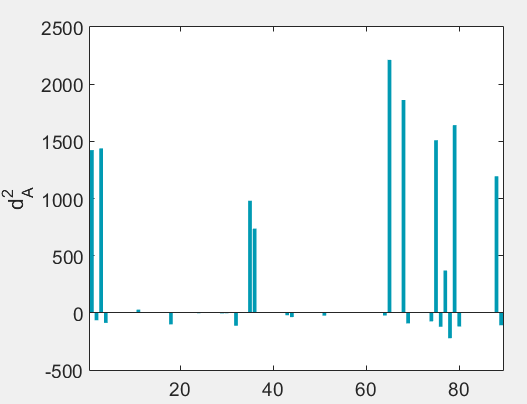
\includegraphics[width=0.7\textwidth]{imagenes/casoEstudio/10_6.png}
\caption{oMEDA de los outliers.}
\end{figure}

\bigskip

En la figura 10.6 se ve el gráfico oMEDA, que relaciona las observaciones interesantes con las variables y se puede apreciar como las variables que mas relación tienen en este grupo de observaciones son 1, 3, 35, 36, 65 , 68, 75, 77, 79 y 88. De las variables anteriores 3, 35 y 77 no se vieron fuertemente relacionadas en MEDA por eso no se mostraron en la tabla 10.1, pero en la tabla 10.2 se pasa a incluirlas.

\bigskip

\begin{table}[H]
\begin{center}
\begin{tabular}{|c|c|c|}
\hline
\textbf{Variable} &\textbf{Nombre} & \textbf{Descripción} \\
 \hline \hline

1 & nf\_sip\_private & IP privada origen\\ \hline
3 & nf\_dip\_private & IP privada destino\\ \hline
35 & nf\_sport\_register & Puerto de origen mayor a 1024 \\ \hline
36 & nf\_sport\_private & Puerto de origen privado \\ \hline
65 & nf\_dport\_8089 & Puerto de destino 8089 \\ \hline
68 & nf\_sport\_register & Puerto de origen mayor a 1024 \\ \hline
75 & nf\_sbyte\_medium & Paquetes de bytes de origen de tamaño medio \\ \hline
77 & nf\_dbyte\_zero & Paquetes de bytes de destino de tamaño pequeño\\	\hline
79 & nf\_dbyte\_medium & Paquetes de bytes de destino de tamaño medio \\ \hline
88 & nf\_state\_close & Estado de conexión cerrado \\ \hline

\end{tabular}
\caption{Contenido variables mostradas en la figura 10.6.}
\end{center}
\end{table}

El gráfico oMEDA nos da una información muy importante para el problema que se está tratando ya que la variable 65 es la que mas altura alcanza y como se ve en la tabla 10.1 esa variable representa al puerto de destino 8089, lo que nos dice que la anomalía probablemente se centra en dicho puerto.

\bigskip

Como los datos con los que se ha realizado el estudio están anonimizados no se puede llegar a obtener la dirección de red ni la dirección física desde donde se esta realizando el ataque, lo que si se puede obtener es el instante de tiempo en el que se a producido.

\bigskip

Para localizar el instante temporal de la anomalía se va a volver a analizar los datos mediante EWMA poniendo como factor de olvido 1.0. Esto hará que cada modelo intermedio que se genere tenga todos los datos de los ficheros anteriores, sin pérdida de información. De esta manera iré comprobando los omeda de todos los puntos de los modelos intermedios y en el momento en el que el uso de la variable 65 se dispare se tendrá localizado el inicio del ataque.
\bigskip

Tras un análisis de las visualizaciones se detecta que es a partir del modelo 4 cuando se comienza el ataque, pasamos a comprobarlo en los gráficos.

\bigskip

\begin{figure}
\centering
\subfigure[Modelo 1]{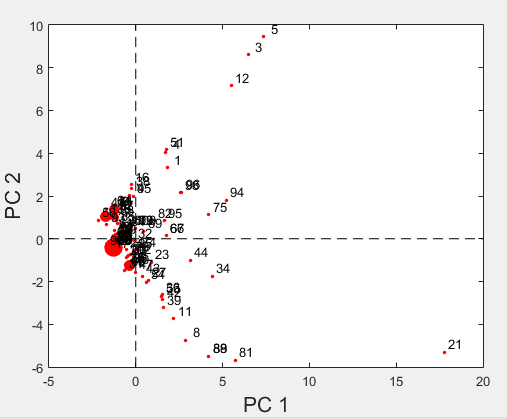
\includegraphics[width=40mm]{imagenes/casoEstudio/10_7_1.png}}
\subfigure[Modelo 2]{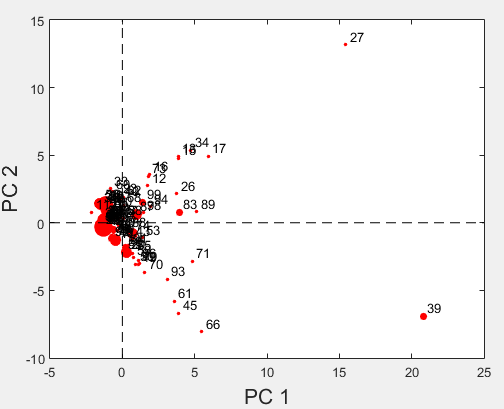
\includegraphics[width=40mm]{imagenes/casoEstudio/10_7_2.png}}
\subfigure[Modelo 3]{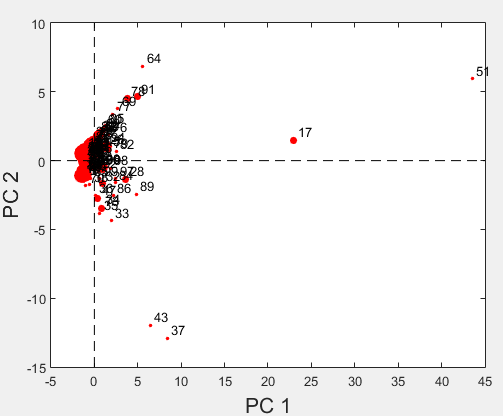
\includegraphics[width=40mm]{imagenes/casoEstudio/10_7_3.png}}
\subfigure[Modelo 4]{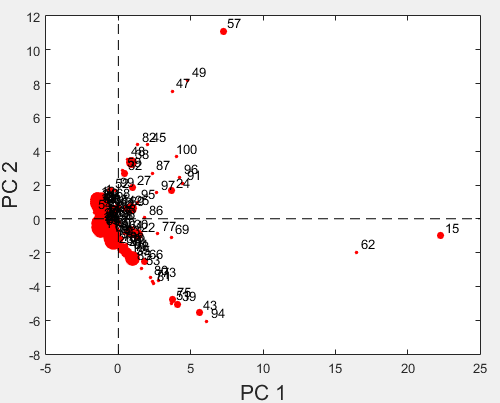
\includegraphics[width=40mm]{imagenes/casoEstudio/10_7_4.png}}
\subfigure[Modelo 5]{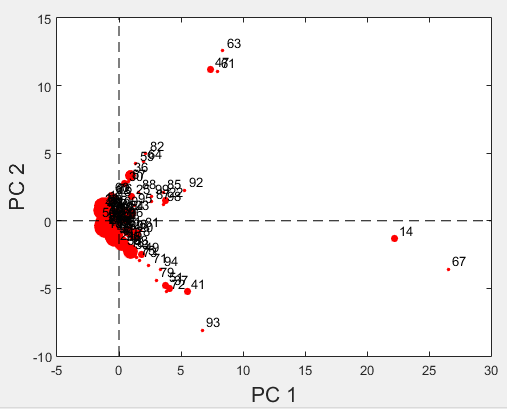
\includegraphics[width=40mm]{imagenes/casoEstudio/10_7_5.png}}
\subfigure[Modelo 6]{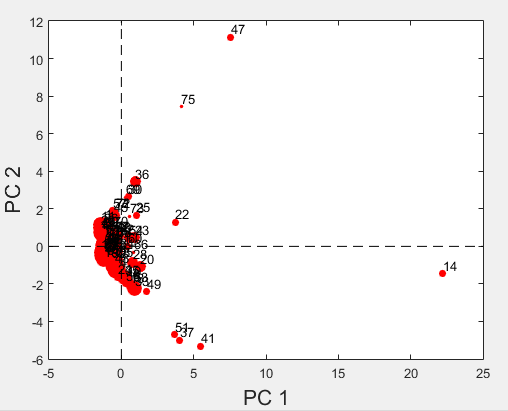
\includegraphics[width=40mm]{imagenes/casoEstudio/10_7_6.png}}
\subfigure[Modelo 7]{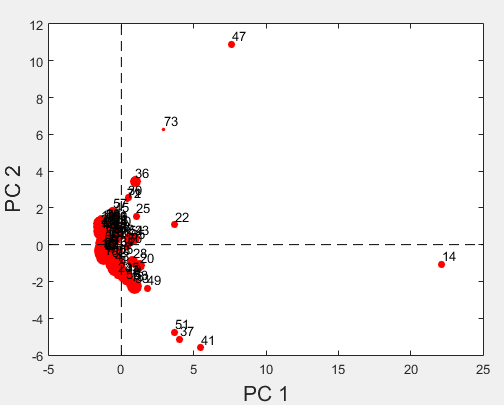
\includegraphics[width=40mm]{imagenes/casoEstudio/10_7_7.png}}
\subfigure[Modelo 8]{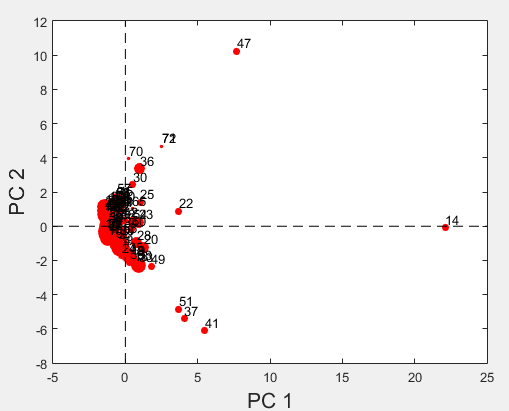
\includegraphics[width=40mm]{imagenes/casoEstudio/10_7_8.png}}
\subfigure[Modelo 9]{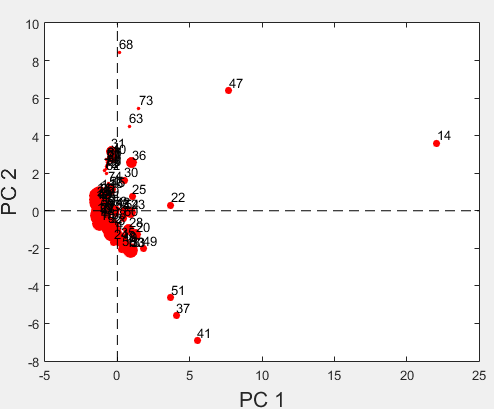
\includegraphics[width=40mm]{imagenes/casoEstudio/10_7_9.png}}
\caption{Score Plots entre modelos 1 y 9.}
\end{figure}

\bigskip

La figura 10.7 muestra la evolución de los Score Plots de los primeros 9 modelos. En dicha figura se puede ver como a partir del modelo 5 aparece un outlier con la etiqueta 14 que aparace en los siguientes gráficos, del cual se va a mostrar el oMEDA.

\begin{figure}
\centering
\subfigure[Modelo 5]{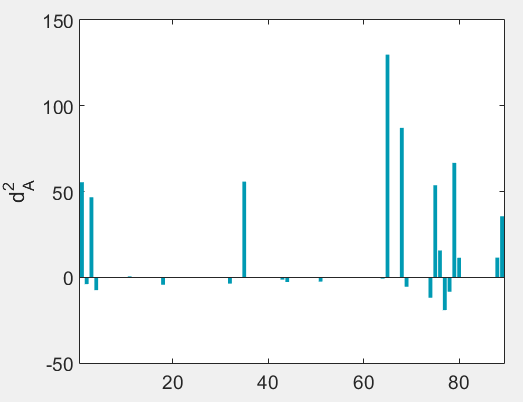
\includegraphics[width=60mm]{imagenes/casoEstudio/10_8_1.png}}
\subfigure[Modelo 6]{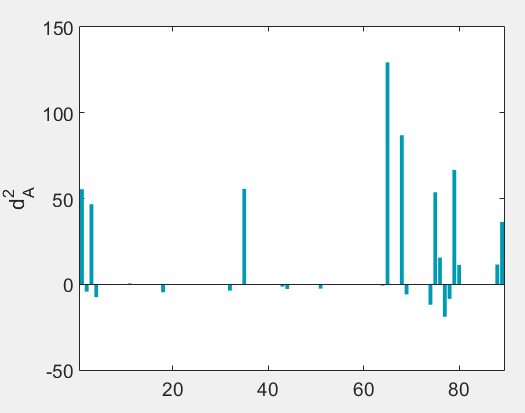
\includegraphics[width=60mm]{imagenes/casoEstudio/10_8_2.png}}
\subfigure[Modelo 7]{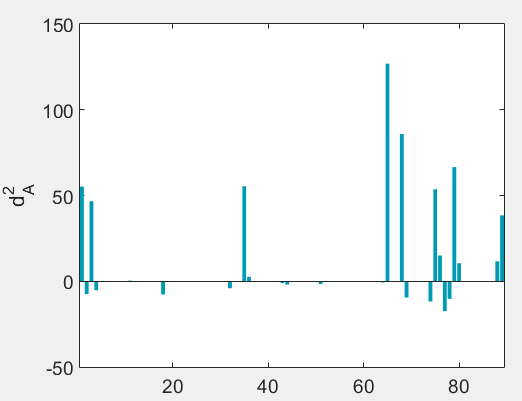
\includegraphics[width=60mm]{imagenes/casoEstudio/10_8_3.png}}
\subfigure[Modelo 8]{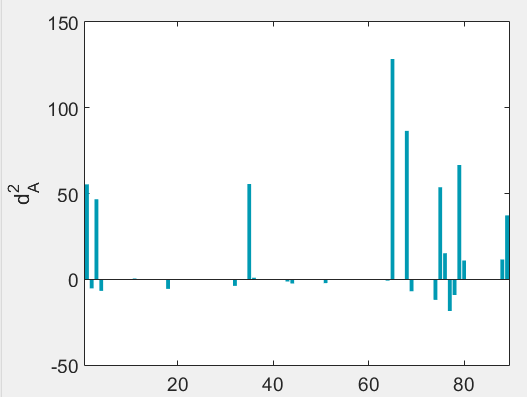
\includegraphics[width=60mm]{imagenes/casoEstudio/10_8_4.png}}
\caption{oMEDA entre modelos 5 y 8 sobre la observarción 14.}
\end{figure}

\bigskip

\begin{table}[H]
\begin{center}
\begin{tabular}{|c|c|c|}
\hline
\textbf{Variable} &\textbf{Nombre} & \textbf{Descripción} \\
 \hline \hline

1 & nf\_sip\_private & IP privada origen\\ \hline
3 & nf\_dip\_private & IP privada destino\\ \hline
35 & nf\_sport\_register & Puerto de origen mayor a 1024 \\ \hline
65 & nf\_dport\_8089 & Puerto de destino 8089 \\ \hline
68 & nf\_sport\_register & Puerto de origen mayor a 1024 \\ \hline
75 & nf\_sbyte\_medium & Paquetes de bytes de origen de tamaño medio \\ \hline
79 & nf\_dbyte\_medium & Paquetes de bytes de destino de tamaño medio \\ \hline
89 & nf\_state\_open & Estado de conexión abierta \\ \hline

\end{tabular}
\caption{Contenido variables mostradas en la figura 10.8.}
\end{center}
\end{table}

Cómo se puede apreciar en la figura 10.8 el outlier comentado se puede identificar con el de la figura 10.5 etiquetado con el número 65 ya que los oMEDA comparten la mayor parte de las variables relevantes mostradas en la tabla 10.2.
\bigskip

Todo esto indica que es en el instante de tiempo del fichero 5 cuando se produce el inicio del ataque. Como los datos fueron previamente anonimizados no podemos identificar la IP del atacante pero se conoce el puerto de ataque, el instante temporal y los tamaños de paquetes que se envían, lo que demuestra que con las herramientas de la MEDA-Toolbox se pueden identificar las anomalías de forma eficaz.